In questa sezione viene data la specifica di quello che \`{e} stato progettatto per ogni incremento, utilizzando un linguaggio discorsivo in cui si spiegano le ragioni e le situazioni che hanno portato a determinate scelte progettuali.
\subsection{Incremento 1}
Il primo incremento consiste nell\textquoteright{}introduzione nella pianificazione delle attivit\`{a} nel riportare il loro inizio e fine alla precisione del minuto. Questa parte di progettazione viene tracciata con il soddisfacimento dei seguenti requisiti:

\begin{longtable}{|>{\centering}p{3cm}|}
    \hline
    \multicolumn{1}{|c|}{\textbf{Requisiti}} \\ %\tabularnewline 
      \hline
        RF.ob.1 \tabularnewline \hline
		RF.ob.1.1 \tabularnewline \hline
		RF.ob.1.2 \tabularnewline \hline
		RF.ob.2 \tabularnewline \hline
		RF.ob.3 \tabularnewline \hline
    \caption{Tracciamento requisiti - Componenti incremento1}
    \label{tab:Tracciamento requisiti - Componenti incremento1}
\end{longtable}

Le classi appartenenti al Model, che memorizzano le informazioni relative alla data di inizio e fine utilizzano, alla versione di OnePointProject scaricabile da sourceforge, un tipo \textit{java.sql.Date}; tuttavia nel database MsSQL la data di inizio e fine vengono salvate con un tipo \textit{datetime}. Quindi per questo incremento \`{e} stato scelto di cambiare il tipo \textit{java.sql.Date} con il tipo \textit{java.sql.Timestamp}, per le seguenti ragioni: data e ora memorizzate in un solo campo del database; data e ora memorizzate in un solo tipo Java; poich\`{e} l\textquoteright{}applicativo nel diagramma di Gantt utilizza per le operazioni la trasformazione della data in millisecondi \`{e} pi\`{u} facile adattare le modifiche cambiando il tipo in un tipo che presenta lo stesso metodo per ottenere i millisecondi. Quindi in questo modo il diagramma di Gantt per durate di attivit\`{a} superiore al giorno visualizzer\`{a} le attivit\`{a} nella posizione corretta rispetto all\textquoteright{}ora del giorno impostato. In questa fase occorrono anche delle modifiche da apportare ai form per l\textquoteright{}inserimento di attivit\`{a} in WBS, permettendo l\textquoteright{}inserimento dell\textquoteright{}ora di inizio e fine oltre che la data; occorre cambiare il tipo di inserimento della durata; il tipo progettato ha nominativo \textit{durationstring}. Per questo nuovo tipo occorre seguire la seguente procedura:
\begin{description}
\item[XComponent.java]: aggiungere \textit{case} per la visualizzazione del componente, per l\textquoteright{}impostazione del valore, per l\textquoteright{}impostazione del tipo di editor, per gli eventi che vedono coinvolto il componente.
\item[XExpressProxy.java]: questa classe svolge la funzione di proxy di protezione per l\textquoteright{}interazione tra file di script (con estensione \textit{jes}) e i metodi delle classi \textit{Java} interessate. In questa classe \`{e} necessario aggiungere i metodi che coinvolgono il tipo interessato. Nel caso del tipo \textit{durationstring} sono stati progettati metodi di set e get del valore che il tipo racchiude.
\item[XDefaultComponentHandler]: questa classe viene utilizzata come classe di \textit{''factory''} per i vari componenti grafici in relazione al tipo; occorre aggiungere il \textit{case} per la creazione di oggetti \textit{XComponent} di tipo \textit{durationstring}.
\end{description}

\subsection{Incremento 2}
Il secondo incremento consiste nella creazione dei componenti necessari per la configurazione delle risorse. Questa parte di progettazione viene tracciata con il soddisfacimento dei seguenti requisiti:

\begin{longtable}{|>{\centering}p{3cm}|}
    \hline
    \multicolumn{1}{|c|}{\textbf{Requisiti}} \\ %\tabularnewline 
      \hline
        RF.ob.5 \tabularnewline \hline
		RF.ob.5.1 \tabularnewline \hline
		RF.ob.5.1.1 \tabularnewline \hline
		RF.ob.5.1.2 \tabularnewline \hline
		RF.ob.5.2 \tabularnewline \hline
		RF.ob.5.3 \tabularnewline \hline
		RF.ob.5.4 \tabularnewline \hline
		RF.ob.5.4.1 \tabularnewline \hline
    \caption{Tracciamento requisiti - Componenti incremento2}
    \label{tab:Tracciamento requisiti - Componenti incremento2}
\end{longtable}

Nello sviluppo di questo incremento \`{e} necessario integrare componenti alla View, al Model e all\textquoteright{}application logic.
In OnePointProject alla versione presa in modifica \`{e} presente un pannello di amministrazione risorse in cui \`{e} possibile impostare i costi interni o esterni per la risorsa. Al pannello in questione \`{e} stato progettata l\textquoteright{}aggiunta di nuove schede per l\textquoteright{}inserimento dei dati richiesti dai requisiti tracciati per questo incremento. Le schede da aggiungere sono 3: una per l\textquoteright{}inserimento delle fascie orarie in cui la risorsa pu\`{o} lavorare con la relativa opzione di ereditarit\`{a} delle fascie orarie dal padre per rispettare i vincoli gerarchici; una per l\textquoteright{}inserimento dei giorni in cui la risorsa non pu\`{o} lavorare e le relative fascie orarie con l\textquoteright{}opzione di ereditariet\`{a} dei giorni e delle fascie di fermo dalla risorsa padre; infine una scheda in cui si pu\`{o} impostare se la risorsa lavori o meno nei giorni festivi. Per le modifiche grafiche \`{e} sufficiente modificare il file \textit{edit\_resource.oxf.xml}.
Nel form in cui vanno inserite le disponibilit\`{a} delle fascie orarie delle risorse \`{e} presente una tabella dalla quale \`{e} possibile effettuare l\textquoteright{}aggiunta di una fascia oraria o rimuovere una fascia selezionata. La gestione degli eventi per questo form \`{e} stata impostata in modo che essa venga attuata direttamente da una classe Java e non da un file di script, si tratta dell\textquoteright{}unico form gestito da OnePoint con la normale procedura; la classe in questione \`{e} \textit{OpEditResourceFormHandler.java}. A questa occorre aggiungere tutti i metodi per la gestione degli eventi ed \`{e} necessario gestire il caso in cui si ha la sovrapposizione di intervalli, ovvero fascie orarie inserite dall\textquoteright{}utente. Analogo \`{e} il comportamento della gestione della scheda per l\textquoteright{}inserimento delle fascie orarie in cui la risorsa \`{e} bloccata, con eccezione del fatto che \`{e} possibile impostare anche il giorno in cui la risorsa \`{e} bloccata. L\textquoteright{}utente pu\`{o} inserire pi\`{u} giorni in cui la risorsa \`{e} impossibilitata nel suo lavoro, il sistema non deve comunque rendere persistenti i dati fino a quando non viene effettuato il salvataggio; quindi \`{e} necessario predisporre in \textit{OpEditResourceFormHandler.java} un campo statico con la seguente firma:\\ \textit{public static Map<Timestamp,XComponent> mappaCalendario}; \\ ovvero la chiave sar\`{a} la data scelta e il valore sar\`{a} un set che rappresenta le fascie orarie; l\textquoteright{}inizializzazione va fatta nel momento in cui viene aperto il form per la gestione di una certa risorsa e tale mappa andr\`{a} inizialmente caricata con i dati presenti nel databasee. La mappa andr\`{a} aggiornata nel momento in cui si cambia data e/o vengono fatte aggiunte e/o rimozioni di fascie orarie. Anche il Model \`{e} stato modificato, in particolare \`{e} stato modificato \textit{OpResource.java}, per maggior chiarezza riporto qui la nuova struttura per rappresentare la risorsa interessata.

\begin{figure}[H]
\begin{center}
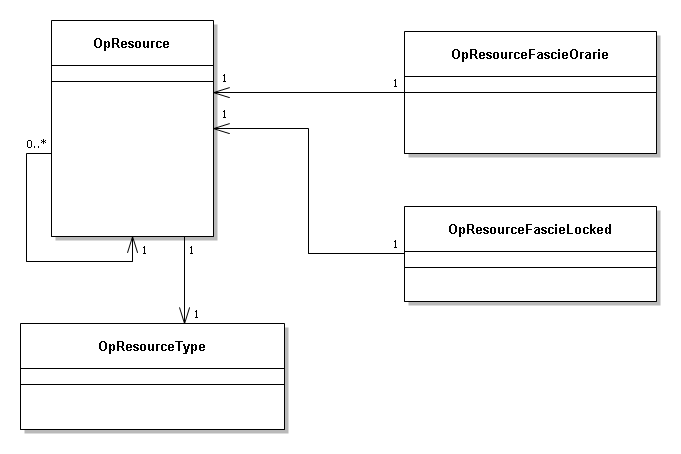
\includegraphics[width=1\textwidth]{img/Resource.png}
\caption{Model: sottocomponente risorsa}
\label{fig:Model: sottocomponente risorsa}
\end{center}
\end{figure}

La seguenta tabella rappresenta i principali attributi caratteristici di una risorsa:
\begin{tabbing}
TABLE \=op\_resource (\\
\>    op\_resourcepool bigint,\\
\>    op\_site bigint,\\
\>    op\_archived bit DEFAULT (0),\\
\>    op\_inheritpoolrate bit,\\
\>    op\_hourlyrate numeric(22, 10),\\
\>    op\_externalrate numeric(22, 10),\\
\>    op\_description varchar(2500),\\
\>    op\_user bigint,\\
\>    op\_inheritfestivita bit, *\\
\>    op\_festivita bit, *\\
\>    op\_inheritfascieorarie bit, *\\
\>    op\_inheritfascielocked bit *,\\
\>    op\_typeresource *\\
);
\end{tabbing}
\textbf{*= add by me} \\ \\
Una risorsa appartiene ad una gerarchia di risorse identificata dall\textquoteright{}attributo op\_resorcepool, che \`{e} una risorsa stessa. Quindi nella relazione sono presenti degli attributi \textit{boolean} (di tipo \textit{bit} in MS Sql) che indicano se l\textquoteright{}entit\`{a} interessata (la risorsa) eredita o meno dalla risorsa padre. Una risorsa pu\`{o} ereditare dal padre i costi, la festivit\`{a}, le fascie orarie, gli impegni della risorsa.
Una risorsa per OnePointProject \`{e} indifferente dal tipo, cio\`{e} una risorsa umana si comporta come una risorsa strumentale. Per CQT e VIDA no, quindi \`{e} stato predisposto un campo op\_resourcetype che si riferisce a una tabella che accumula i tipi della risorsa disponibile.
L\textquoteright{}aggiunta di un tipo comporta un aggiustamento del calcolo. Per ora il calcolo viene effettuatato considerando risorse umane e strumentali.

\subsection{Incremento 3}
Il terzo incremento prevede la gestione del calcolo della durata delle attivit\`{a} in relazione al WBS pianificato. Questa parte di progettazione viene tracciata con il soddisfacimento dei seguenti requisiti:

\begin{longtable}{|>{\centering}p{3cm}|}
    \hline
    \multicolumn{1}{|c|}{\textbf{Requisiti}} \\ %\tabularnewline 
      \hline
        RF.ob.4 \tabularnewline \hline
		RF.ob.4.1 \tabularnewline \hline
		RF.ob.4.1.1 \tabularnewline \hline		
		RF.ob.4.1.1.1 \tabularnewline \hline
		RF.ob.4.1.1.2 \tabularnewline \hline
		RF.ob.4.1.1.3 \tabularnewline \hline
		RF.ob.4.1.2 \tabularnewline \hline
		RF.ob.4.1.2.1 \tabularnewline \hline
		RF.ob.4.1.2.2 \tabularnewline \hline
		RF.ob.4.1.2.2.1 \tabularnewline \hline
		RF.ob.4.1.2.2.2 \tabularnewline \hline
		RF.ob.4.1.3 \tabularnewline \hline
    \caption{Tracciamento requisiti - Componenti incremento3}
    \label{tab:Tracciamento requisiti - Componenti incremento3}
\end{longtable}

Il calcolo viene effettuato nel momento in cui l\textquoteright{}utente decide di effettuare un\textquoteright{}operazione di salvataggio. Viene effettuato, quindi eventualmente aggiornato nel momento in cui, viene cambiata la data di inizio o di fine di un\textquoteright{}attivit\`{a}, quindi la durata, oppure nel momento in cui viene fatta una modifica agli assegnamenti delle attivit\`{a}, modificandoli eliminandoli o inserendone di nuovi. Per fare ci\`{o} nel pi\`{u} semplice modo possibile occorre aggiungere al metodo di salvataggio gi\`{a} previsto dall\textquoteright{}applicativo il metodo con la seguente firma: \\
\textit{eseguiCalcolo(OpBroker broker,OpProjectSession session,OpProjectPlanVersion project);} \\
Un oggetto di tipo \textit{OpBroker} viene utilizzato quando sono necessarie operazioni con il database; la classe \textit{OpBroker.java} presenta metodi per effettuare query e operazioni di CRUD su ennuple e quindi su oggetti. Un oggetto di tipo \textit{OpProjectSession} \`{e} necessario per aprire transazioni e svolge il ruolo di sessione vera e propria ovvero identifca l\textquoteright{}utente autenticato al sistema. Un oggetto di tipo \textit{OpProjectPlanVersion} al fine di identificare il progetto in modifica; con un diagramma delle classi cercher\`{o} di spiegare la funzionalit\`{a} delle classi che sono etichettate con la parola \textit{''Version''}.

\begin{landscape}
\begin{figure}[H]
\begin{center}
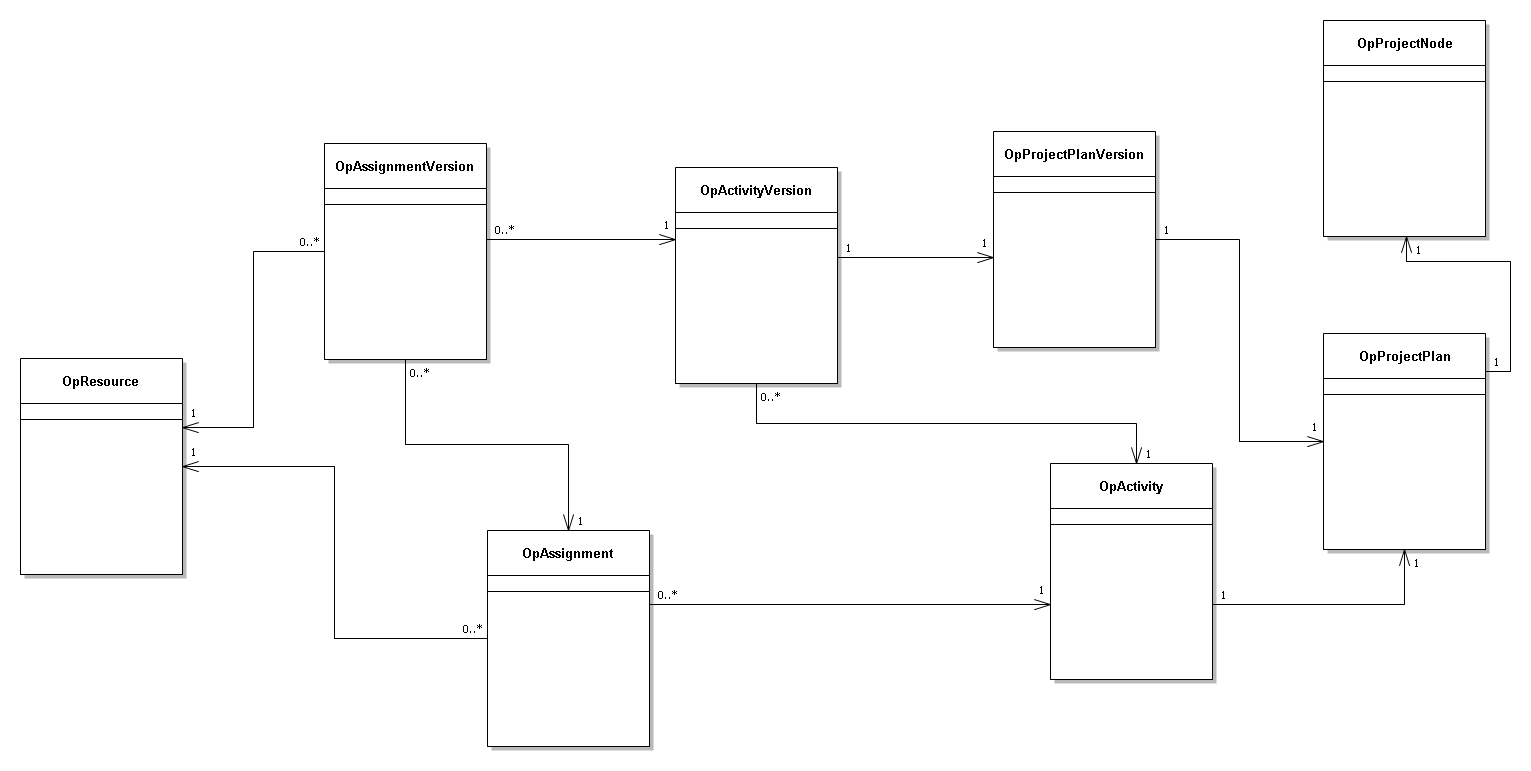
\includegraphics[width=1.6\textwidth]{img/ModelIncremento3.png}
\caption{Model: sottocomponente versionamento}
\label{fig:Model: sottocomponente versionamento}
\end{center}
\end{figure}
\end{landscape}.

Il versionamento delle attivit\`{a} non funziona come un repository. La funzionalit\`{a} \`{e} quella di rendere visibili a tutti le informazioni del progetto all\textquoteright{}ultimo ''check-in'' effettuato, in questo modo se un utente sta modificando il progetto le sue modifiche non verranno viste da tutti fino al suo prossimo ''check-in''. In pratica si tratta di lock in scrittura e la lettura \`{e} permessa all\textquoteright{}ultima versione creato con l\textquoteright{}ultimo ''check-in''.
Nel momento in cui viene effettuata una operazione di salvataggio viene creato un oggetto di tipo \textit{OpActivityVersion} o al massimo esso viene aggiornato, sempre all\textquoteright{}ultima versione ovviamente. Quando si effettua il ''check-in'' viene a crearsi un oggetto di tipo \textit{OpActivity}, che \`{e} la copia di ci\`{o} che \`{e} riportato in \textit{OpActivityVersion} all\textquoteright{}ultima versione in moodifica del piano di progetto.
Un oggetto di tipo \textit{OpProjectPlan} viene creato nel momento in cui si crea un oggetto di tipo \textit{OpProjectNode}, quindi esister\`{a} sempre almeno un oggetto di tipo \textit{OpProjectPlan} riferito al nuovo progetto. Nel momento in cui si salvano le prime attivit\`{a} si crea anche un oggetto di tipo \textit{OpProjectPlanVersion}. Il versionamento \`{e} previsto anche per gli assegnamenti delle risorse alle attivit\`{a}, quindi \`{e} presente una classe \textit{OpAssignment.java} e una classe \textit{OpAssignmentVersion.java}.\\
L\textquoteright{}algoritmo che effettua il calcolo della durata effettiva delle attivit\`{a} necessita dell\textquoteright{}introduzione di una nuova relazione e quindi una nuova classe, \textit{OpAssignmentFascie.java} la cui funzionalit\`{a} \`{e} quello di rappresentare un modello di dati per le fascie orarie in cui una determinata risorsa assegnata ad una certa attivit\`{a} effettua il lavoro. In OnePointProject gli assegnamenti di una risorsa ad un certa attivit\`{a} vengono rappresentati con oggetti di tipo \textit{OpAssignment} e quindi \textit{OpAssignmentVersion}; la nuova relazione creata necessita solo delle informazioni relative a \textit{OpAssignmentVersion}. Infatti l\textquoteright{}algoritmo deve essere applicato acquisendo un ''lock'' sulla scrittura nella relazione OpAssignmentFascie, ovvero l\textquoteright{}esecuzione del calcolo dell\textquoteright{}algoritmo non potr\`{a} mai essere eseguito contemporaneamente su pi\`{u} di 1 progetto; questo perch\`{e} l\textquoteright{}algoritmo controlla se la risorsa \`{e} occupata da altri pogetti in una medesima fascia oraria, quindi se pi\`{u} salvataggi su progetti diversi sono in esecuzione la situazione finale genera un calcolo non veritiero in caso di assenza di ''lock''. Inoltre per le stesse ragioni il salvataggio dovr\`{a} considerare gli assegnamenti inseriti sempre all\textquoteright{}ultima versione per cui \`{e} stato fatta l\textquoteright{}operazione di salvataggio e non all\textquoteright{}ultima versione per cui \`{e} stato fatto il ''check-in''. Quindi nel momento in cui dopo aver effettuto l\textquoteright{}operazione di ''check-in'' si entra in modifica nel progetto, OnePointProject effettua la creazione di nuovi oggetti versionati, quindi gli oggetti coinvolti presenteranno il tipo di \textit{OpProjectPlanVersion, OpActivityVersion, OpAssignmentVersion,} che sono la copia degli oggetti presenti all\textquoteright{}ultimo ''check-in''; le nuove modifiche che verranno salvate verranno salvate su questi oggetti appositamente creati. Occorre tuttavia apportare anche degli aggiornamenti alle ennuple presenti nell\textquoteright{}entit\`{a} \textit{OpAssignmentFascie}; infatti poich\`{e} l\textquoteright{}algoritmo controlla le fascie orarie degli assegnamenti inseriti all\textquoteright{}ultima versione di progetto occorre aggiornare gli assegnamenti inseriti nell\textquoteright{}entit\`{a} \textit{OpAssignmentFascie} con gli identificativi degli assegnamenti creati entrando in modifica nel progetto. Di seguito riporto l\textquoteright{}algoritmo che dovr� essere applicato per effettuare il calcolo con la precisione espressa nei requisiti.
 
\newpage
\begin{lstlisting}[caption={Algoritmo che calcola la durata delle attivit\`{a}}]
//acquisizione lock
//activityPlanVersion ha tipo Iterator e contiene le attivit� del progetto all'ultimo versionamento
while (activityPlanVersion.hasNext()){
	OpActivityVersion activityVersion=activityPlanVersion.next();
	//creazione di una mappa che presenta come chiave la risorsa e come valore l'impegno residuo della risorsa
	HashMap<OpResource,Double>resources = new HashMap<OpResource,Double>();
	//assignmentsVersion ha tipo Iterator e contiene gli assegnamenti predisposti per l'attivit� activityVersion
	if (assignmentsVersion.hasNext){
		while (assignmentsVersion.hasNext()){
			OpResource resource=assignmentsVersion.next();
			resources.put(resource,resource.getBaseEffort());
		}
		//salvataggio nella variabile time l'ora di inizio dell'attivit�
		Timestamp time=new Timestamp(activityVersion.getStart().getTime();)
		Integer durata=0;
		//il ciclo continua fino a quando esiste almeno una risorsa il cui impegno residuo � maggiore di 0
		while (remainingEffort(resources)){
			//selezionare le risorse disponibili in base ai requisiti fissati
			Collection<OpResource> resourcesAvailable=getResourceAvailable(broker,time,
			resources.keySet,planVersion,activityVersion);
			//diminuire l'impegno delle risorse in base al loro tipo, eliminando eventualmente le risorse se hanno colmato l'impegno
			OpResourceCalcoloHelper.diminuisciEffort(resourcesAvailable,
			resources);
			//aggiornamento per le risorse disponibili l'occupazione nel tempo time
			durata++;
			time=new Timestamp(time.getTime()+1000*60);
		}
		//modifica della data di fine in base alla durata calcolata
		updateFine(activityVersion,durata);
	}
}	
//unlock
\end{lstlisting}

Per rendere il pi\`{u} indipendente possibile la relazione tra l\textquoteright{}algoritmo e il tipo delle risorse \`{e} stata introdotta la classe \textit{OpResourceCalcoloHelper.java} la cui utilit\`{a} \`{e} di richiamare il metodo opportuno di diminuzione dell\textquoteright{}impegno residuo in base al tipo della risorsa.

\newpage
\subsection{Incremento 4}
Il quarto incremento consiste nella possibilit\`{a} di modificare graficamente il diagramma di Gantt e di apportare modifiche al WBS nel caso in cui venga modificata la durata delle attivit\`{a} del diagramma di Gantt, con incrementi o decrementi di durata inferiore alle 24 ore. Questa parte di progettazione viene tracciata con il soddisfacimento dei seguenti requisiti:

\begin{longtable}{|>{\centering}p{3cm}|}
    \hline
    \multicolumn{1}{|c|}{\textbf{Requisiti}} \\ %\tabularnewline 
      \hline
        RF.de.1 \tabularnewline \hline
		RF.de.2 \tabularnewline \hline
		RF.de.3 \tabularnewline \hline
		RF.de.3.1 \tabularnewline \hline
		RF.de.3.2 \tabularnewline \hline
    \caption{Tracciamento requisiti - Componenti incremento4}
    \label{tab:Tracciamento requisiti - Componenti incremento4}
\end{longtable}